% Options for packages loaded elsewhere
\PassOptionsToPackage{unicode}{hyperref}
\PassOptionsToPackage{hyphens}{url}
\documentclass[
]{book}
\usepackage{xcolor}
\usepackage{amsmath,amssymb}
\setcounter{secnumdepth}{5}
\usepackage{iftex}
\ifPDFTeX
  \usepackage[T1]{fontenc}
  \usepackage[utf8]{inputenc}
  \usepackage{textcomp} % provide euro and other symbols
\else % if luatex or xetex
  \usepackage{unicode-math} % this also loads fontspec
  \defaultfontfeatures{Scale=MatchLowercase}
  \defaultfontfeatures[\rmfamily]{Ligatures=TeX,Scale=1}
\fi
\usepackage{lmodern}
\ifPDFTeX\else
  % xetex/luatex font selection
\fi
% Use upquote if available, for straight quotes in verbatim environments
\IfFileExists{upquote.sty}{\usepackage{upquote}}{}
\IfFileExists{microtype.sty}{% use microtype if available
  \usepackage[]{microtype}
  \UseMicrotypeSet[protrusion]{basicmath} % disable protrusion for tt fonts
}{}
\makeatletter
\@ifundefined{KOMAClassName}{% if non-KOMA class
  \IfFileExists{parskip.sty}{%
    \usepackage{parskip}
  }{% else
    \setlength{\parindent}{0pt}
    \setlength{\parskip}{6pt plus 2pt minus 1pt}}
}{% if KOMA class
  \KOMAoptions{parskip=half}}
\makeatother
\usepackage{color}
\usepackage{fancyvrb}
\newcommand{\VerbBar}{|}
\newcommand{\VERB}{\Verb[commandchars=\\\{\}]}
\DefineVerbatimEnvironment{Highlighting}{Verbatim}{commandchars=\\\{\}}
% Add ',fontsize=\small' for more characters per line
\usepackage{framed}
\definecolor{shadecolor}{RGB}{248,248,248}
\newenvironment{Shaded}{\begin{snugshade}}{\end{snugshade}}
\newcommand{\AlertTok}[1]{\textcolor[rgb]{0.94,0.16,0.16}{#1}}
\newcommand{\AnnotationTok}[1]{\textcolor[rgb]{0.56,0.35,0.01}{\textbf{\textit{#1}}}}
\newcommand{\AttributeTok}[1]{\textcolor[rgb]{0.13,0.29,0.53}{#1}}
\newcommand{\BaseNTok}[1]{\textcolor[rgb]{0.00,0.00,0.81}{#1}}
\newcommand{\BuiltInTok}[1]{#1}
\newcommand{\CharTok}[1]{\textcolor[rgb]{0.31,0.60,0.02}{#1}}
\newcommand{\CommentTok}[1]{\textcolor[rgb]{0.56,0.35,0.01}{\textit{#1}}}
\newcommand{\CommentVarTok}[1]{\textcolor[rgb]{0.56,0.35,0.01}{\textbf{\textit{#1}}}}
\newcommand{\ConstantTok}[1]{\textcolor[rgb]{0.56,0.35,0.01}{#1}}
\newcommand{\ControlFlowTok}[1]{\textcolor[rgb]{0.13,0.29,0.53}{\textbf{#1}}}
\newcommand{\DataTypeTok}[1]{\textcolor[rgb]{0.13,0.29,0.53}{#1}}
\newcommand{\DecValTok}[1]{\textcolor[rgb]{0.00,0.00,0.81}{#1}}
\newcommand{\DocumentationTok}[1]{\textcolor[rgb]{0.56,0.35,0.01}{\textbf{\textit{#1}}}}
\newcommand{\ErrorTok}[1]{\textcolor[rgb]{0.64,0.00,0.00}{\textbf{#1}}}
\newcommand{\ExtensionTok}[1]{#1}
\newcommand{\FloatTok}[1]{\textcolor[rgb]{0.00,0.00,0.81}{#1}}
\newcommand{\FunctionTok}[1]{\textcolor[rgb]{0.13,0.29,0.53}{\textbf{#1}}}
\newcommand{\ImportTok}[1]{#1}
\newcommand{\InformationTok}[1]{\textcolor[rgb]{0.56,0.35,0.01}{\textbf{\textit{#1}}}}
\newcommand{\KeywordTok}[1]{\textcolor[rgb]{0.13,0.29,0.53}{\textbf{#1}}}
\newcommand{\NormalTok}[1]{#1}
\newcommand{\OperatorTok}[1]{\textcolor[rgb]{0.81,0.36,0.00}{\textbf{#1}}}
\newcommand{\OtherTok}[1]{\textcolor[rgb]{0.56,0.35,0.01}{#1}}
\newcommand{\PreprocessorTok}[1]{\textcolor[rgb]{0.56,0.35,0.01}{\textit{#1}}}
\newcommand{\RegionMarkerTok}[1]{#1}
\newcommand{\SpecialCharTok}[1]{\textcolor[rgb]{0.81,0.36,0.00}{\textbf{#1}}}
\newcommand{\SpecialStringTok}[1]{\textcolor[rgb]{0.31,0.60,0.02}{#1}}
\newcommand{\StringTok}[1]{\textcolor[rgb]{0.31,0.60,0.02}{#1}}
\newcommand{\VariableTok}[1]{\textcolor[rgb]{0.00,0.00,0.00}{#1}}
\newcommand{\VerbatimStringTok}[1]{\textcolor[rgb]{0.31,0.60,0.02}{#1}}
\newcommand{\WarningTok}[1]{\textcolor[rgb]{0.56,0.35,0.01}{\textbf{\textit{#1}}}}
\usepackage{longtable,booktabs,array}
\newcounter{none} % for unnumbered tables
\usepackage{calc} % for calculating minipage widths
% Correct order of tables after \paragraph or \subparagraph
\usepackage{etoolbox}
\makeatletter
\patchcmd\longtable{\par}{\if@noskipsec\mbox{}\fi\par}{}{}
\makeatother
% Allow footnotes in longtable head/foot
\IfFileExists{footnotehyper.sty}{\usepackage{footnotehyper}}{\usepackage{footnote}}
\makesavenoteenv{longtable}
\usepackage{graphicx}
\makeatletter
\newsavebox\pandoc@box
\newcommand*\pandocbounded[1]{% scales image to fit in text height/width
  \sbox\pandoc@box{#1}%
  \Gscale@div\@tempa{\textheight}{\dimexpr\ht\pandoc@box+\dp\pandoc@box\relax}%
  \Gscale@div\@tempb{\linewidth}{\wd\pandoc@box}%
  \ifdim\@tempb\p@<\@tempa\p@\let\@tempa\@tempb\fi% select the smaller of both
  \ifdim\@tempa\p@<\p@\scalebox{\@tempa}{\usebox\pandoc@box}%
  \else\usebox{\pandoc@box}%
  \fi%
}
% Set default figure placement to htbp
\def\fps@figure{htbp}
\makeatother
\setlength{\emergencystretch}{3em} % prevent overfull lines
\providecommand{\tightlist}{%
  \setlength{\itemsep}{0pt}\setlength{\parskip}{0pt}}
\usepackage[]{natbib}
\bibliographystyle{plainnat}
\usepackage{booktabs}
\usepackage{bookmark}
\IfFileExists{xurl.sty}{\usepackage{xurl}}{} % add URL line breaks if available
\urlstyle{same}
% fallback for those not using the hyperref driver hyperxmp:
\makeatletter
\@ifundefined{xmpquote}{\newcommand{\xmpquote}[1]{#1}}{}
\makeatother
\hypersetup{
  pdftitle={EcoMods Booklet},
  pdfauthor={The EcoMods, Würzburg},
  hidelinks,
  pdfcreator={LaTeX via pandoc}}

\title{EcoMods Booklet}
\author{The EcoMods, Würzburg}
\date{2026-11-11}

\begin{document}
\maketitle

{
\setcounter{tocdepth}{1}
\tableofcontents
}
\chapter{About this book}\label{about-this-book}

Hello and welcome to the EcoMods working group!

In this document, you will (hopefully) find everything you need for your course / internship / thesis with us.

The book is meant to be a live document, and will be updated
continuously. As you browse through sections, you will encounter empty
or incomplete sections. You're welcome to ask for sections to be added,
updated, or even better, improve it yourself! See section
\ref{contributing}.

\section{Acknowldegements and licensing}\label{acknowldegements-and-licensing}

This manual is an update of a manual of the \href{CCTB-Ecomods/Ecomods-Booklet}{original
Ecomods} at the University of Würzburg.
Huge thanks to them for assembling this knowledge base!

The manual is published under the terms of the \href{https://github.com/biob-ecomod/ecomods_booklet/blob/main/LICENSE}{MIT
License},
which means you can freely copy, modify and share its contents as long
as you acknowledge the original work and provide a copyright notice and
copy in the license in all derived works.

\section{Contributing to this book}\label{contributing-to-this-book}

We gladly accept any suggestions on how to improve this guide, so let us
know if you feel that anything is missing!

This booklet is a bookdown document. This means, that it consists of
several R Markdown files. To learn R markdown see section \ref{rmd}.
The booklet is hosted on
\href{https://github.com/CCTB-Ecomods/Ecomods-Booklet}{GitHub} (see section
\ref{version-control}.

\begin{enumerate}
\def\labelenumi{\arabic{enumi}.}
\item
  Step: Clone the repository from GitHub.
\item
  Step: Open the .rmd file of the Chapter you would like to change.
\item
  Step: Do your changes.
\item
  Step: Commit your changes and push them on GitHub.
\item
  Step: Then the magic happens: via github actions the website will be
  updated, but this takes 5-10 Minutes (check the green dot!). This
  creates files that are pushed automatically. Therefore, don't work
  within the Repo while waiting and \textbf{pull the changes} before you go
  on editing.
\end{enumerate}

Don't forget to add links, citations, figures etc in a nice and
organized way. Check text for typos and readability and be sure that a
beginner can understand it.

\section{Missing sections and TODOs within this booklet}\label{missing-sections-and-todos-within-this-booklet}

If you find any missing topics, collect them here or write a \emph{TODO} at
the appropriate part.

\section{People}\label{people}

{[}TODO{]}

\section{Induction}\label{induction}

Welcome to the group! We hope you have a great time with us and that
your experience in your lab will be the opportunity to develop your
academic skills and explore exciting research!

Here are some things you should consider upon joining us:

\begin{itemize}
\item
  \textbf{🔑 Keys}: our lab is hosted in the old NEES institute,
  \href{https://www.openstreetmap.org/way/406460211}{Venusbergweg 22}, at the
  edge of the Botanische Gärten. Access to the building and other
  facilities of the institute is managed through transponders, which you
  must obtain in person from Elke Friesecke at the main building of the
  Nees-Institut (\href{https://www.openstreetmap.org/way/149556476}{Meckenheimer Allee
  170}). You will need to
  return the transponders upon leaving.
\item
  \textbf{🔘 Slack}: we have a Slack workspace for the group, which is our
  main channel for communication. You will find links to the lab meeting
  schedule and zoom call pinned in the \#general channel. Ask another
  team member for an invite link!
\item
  \textbf{🗨️ Whatsapp}: we have a Whatsapp convo for instant communication
  (mostly socials). Ask a team member for an invite if you'd like to
  join.
\item
  \textbf{📆 Calendar}: We keep a Google Calendar to pin and share relevant
  events. If you'd like to get access, send a google account address to
  Theo.
\item
  \textbf{👥 Meetings}: save these time slots for regular meetings:

  \begin{itemize}
  \tightlist
  \item
    Weekly Ecomod lab meeting, Mondays 17:00-18:00.
  \item
    NEES seminar (jointly with Prof.~Max Weigend's group) Tuesdays
    16:30-17:30
  \end{itemize}
\end{itemize}

The schedule for the lab meetings is available
\href{https://docs.google.com/document/d/1p0EdFmez05UcZ4QUoacWM9PfAQuAKpg7XM1HtXeEdRU/edit?usp=sharing}{here}.
It is also possible to join online, the zoom link is pinned in the
Slack's general channel.

\begin{itemize}
\item
  \textbf{🤖 IT questions:} Theo can help with all research-related software
  enquiries. For hardware issues, the responsible person for BIOB is
  Tomislav Balen. In particular, for security reasons our printer can
  only be accessed with specific drivers, which are to be installed by
  Tomi.
\item
  \textbf{📖 University Library:} before using the services of the ULB
  (Universitäts und Landesbibliothek Bonn), you will need to get
  yourself a library ID card (Bibliothekausweis) and a user account,
  which are not automatically created upon joining the University. The
  procedure is detailed on the \href{https://www.ulb.uni-bonn.de/de/nutzung-und-ausleihe/ausweis-konto}{ULB
  website}.
  You will need to submit a form, get the Uni Bonn app and after a few
  days you will receive instructions on how to link your Uni-ID into the
  app. Finally, you will need to head to the main ULB building to show a
  piece of ID, proof of residence and proof of affiliation with Uni Bonn
  (enrolment certificate or work contract).
\end{itemize}

\section{What you can find in this booklet}\label{what-you-can-find-in-this-booklet}

You'll find information about the following topics:

\begin{itemize}
\item
  \textbf{Programming tools} in Chapter \ref{programming-tools}
\item
  \textbf{IT infrastructure} in Chapter \ref{it-infrastructure}
\item
  \textbf{Process based models} in Chapter \ref{process-based-models}
\item
  \textbf{Computational methods} in Chapter \ref{computational-methods}
\item
  \textbf{Project management} in Chapter \ref{project-management}
\item
  \textbf{Writing \& Publishing} in Chapter \ref{writing-publishing}
\end{itemize}

\chapter{Programming tools}\label{programming-tools}

\section{Basic tools and languages}\label{basic-tools-and-languages}

The most commonly used programming languages in our lab are R and Julia.
They are both great languages for biology-related programming and
statistical analysis.

If you already know how to program and are looking for a challenge, our
lab members enjoy participating in \href{https://adventofcode.com/}{Advent of
Code}. It forces you to think outside the box
and will teach you some new tricks!

\subsection{R}\label{r}

\href{https://www.r-project.org/}{R} is very well-established and probably
has the most support from all the languages we use. Most of the time,
you can copy-paste your error message from R into Google, and you will
find several solutions for your problem. A very helpful website is
\href{https://stackoverflow.com/}{Stack Overflow}.

\subsubsection{Interface}\label{interface}

In our lab, most people use \href{https://www.rstudio.com/}{RStudio} when
they are working in R. RStudio allows you to very easily write and
execute your scripts, create plots and keep an eye on your environment.
It also includes a helpful debugging mode. Other, not as commonly used
GUIs are \href{https://rkward.kde.org/}{RKWard},
\href{https://www.blueskystatistics.com/Default.asp}{BlueSky} and \href{https://socialsciences.mcmaster.ca/jfox/Misc/Rcmdr/}{R
Commander}.

\subsubsection{Resources}\label{resources}

To get started, there are several books on how to use R.

\href{https://r4ds.had.co.nz/}{R for Data Science}: ``You'll learn how to get
your data into R, get it into the most useful structure, transform it,
visualise it and model it.''

\href{https://adv-r.hadley.nz/}{Advanced R}: ``The book is designed primarily
for R users who want to improve their programming skills and
understanding of the language. It should also be useful for programmers
coming to R from other languages, as help you to understand why R works
the way it does.''

Further reading:

\begin{itemize}
\item
  Coding Etiquette (in R) - slides from \emph{Anne} prepared for BioInfo F2
  2020 (ask Anne)
\item
  Troubleshooting in R - Slides from \emph{Anne} prepared for BioInfo F2
  2020 (ask Anne)
\item
  R for Dummies, Andrie de Vries \& Joris Meys, 2015 (PDF available,
  ask Jana)
\end{itemize}

\subsubsection{Packages}\label{packages}

What are \href{https://r-pkgs.org/}{R packages}?

If you have a problem that you need a certain function to solve, many
times you do not need to write that function from scratch yourself.
Usually, another (more skilled) person has already written some code
that solves this problem. These ``packages of code'' can be uploaded to
CRAN (the Comprehensive R Archive Network) and then downloaded to be
used by other users.

An example: You have a nice plot and want to ensure it is easy to read
and interpret for colorblind people. Now you could set all of your 200
colors by hand so that it is not the default red-green nightmare, but it
is much easier to just download a package called ``viridis'' that contains
multiple color palettes that are optimized for this very use. Then, all
you need to do is tell R to use the viridis palette instead of setting
all colors by hand, which would get very tedious. Installing and loading
a package via CRAN:

\begin{verbatim}
install.packages("PackageName")
library(PackageName)
\end{verbatim}

Note that packages need to be loaded into your environment using the
\texttt{library()} command in order for R to use them. You can also download
packages that are not yet on CRAN using
\href{https://www.r-project.org/nosvn/pandoc/devtools.html}{devtools}.

Commonly used packages in our working group include (but are not limited
to):

\begin{itemize}
\item
  \href{https://www.tidyverse.org/}{tidyverse}
\item
  \href{https://here.r-lib.org/}{here}
\item
  \href{https://www.r-project.org/nosvn/pandoc/devtools.html}{devtools}
\item
  \href{https://ggplot2.tidyverse.org/}{ggplot2}
\item
  \href{https://cran.r-project.org/web/packages/viridis/vignettes/intro-to-viridis.html}{viridis}
\item
  \href{https://cran.r-project.org/web/packages/raster/index.html}{raster}
\item
  \href{https://cran.r-project.org/web/packages/rgdal/index.html}{rgdal}
\end{itemize}

\subsubsection{Rmd}\label{rmd}

R Markdown is a great way to create documents in HTML, Word or PDF
format. Rmds can include chunks of code which create the tables and
plots of the document. This way, you don't have to update your document
parallel to your code, as you keep both your code to create your plots
and said plots in the file. This file was also created using Rmd! You
can also use .Rmd files to create computational notebooks.

\href{https://bookdown.org/yihui/rmarkdown/}{Best overall guide} is linked.

A future alternative might be \href{https://quarto.org/}{quarto}.

\subsection{Julia, the language}\label{julia-the-language}

\href{https://julialang.org/}{Julia} is a relatively new programming language
with a significantly higher performance than R. For complex models that
take a lot of time to run in R, it might make sense to transfer them to
Julia. While it has many advantages, it is not as well-known as R, so
you may need to search for an explanation for your error message a bit
longer. Julia has its own \href{https://discourse.julialang.org/}{Discourse}
page with many helpful entries and tutorials as well.

The Julia \href{https://docs.julialang.org/en/v1/}{Documentation} is also
VERY good.

To quickly look up Julia syntax, you can use this \href{https://juliadocs.github.io/Julia-Cheat-Sheet/}{Cheat
Sheet}.

\subsubsection{Best tutorials}\label{best-tutorials}

To get started,
\href{https://benlauwens.github.io/ThinkJulia.jl/latest/book.html}{here} is a
very nice book for beginners by Ben Lauwens and Allen Downey that
explains not only the Julia language, but also introduces the concept of
programming in general.

\href{https://juliaacademy.com/courses}{JuliaAcademy} offers an introductory
course that is tried and liked by Robin.

If you are not that into reading, the official Julia Programming
Language \href{https://www.youtube.com/channel/UC9IuUwwE2xdjQUT_LMLONoA}{Youtube
channel} has
some very nice tutorials structured by playlists. One especially helpful
playlist is \href{https://www.youtube.com/watch?v=ub3tqCWZmo4&list=PLP8iPy9hna6Qpx0MgGyElJ5qFlaIXYf1R}{Julia Programming for Nervous
Beginners}.
They also hold the annual \href{https://juliacon.org/2022/}{JuliaCon} online
and upload the speaker's talks to Youtube if you cannot be there live.

\subsubsection{Plotting in Julia}\label{plotting-in-julia}

Plots in Julia can be a bit more tricky than in R (but that might be
because we are used to plotting in R - don't let this discourage you
from plotting your heart out in Julia if that is what you want to do!).
Here are some packages that may help facilitate your plotting
adventures:

\begin{itemize}
\item
  \href{https://juliapackages.com/c/graphical-plotting}{This} page shows a
  list of graphical plotting packages
\item
  \href{https://makie.juliaplots.org/stable/}{GLMakie} is used by \emph{Robin}
\end{itemize}

\subsubsection{Interface}\label{interface-1}

As for R, you can choose from a variety of interfaces for Julia. In our
working group, these are the most common ones:

\begin{itemize}
\item
  \href{https://junolab.org/}{Atom and Juno} for julia.
  \href{https://techytok.com/atom-and-juno-setup-for-julia/}{Here} is a
  nice tutorial on how to set it up. However, even though popular in
  our lab, Juno will receive no more feature updates as of March 2022,
  so if you are new to Julia, it might be best to choose a different
  IDE.
\item
  \href{https://www.julia-vscode.org/}{VSCode} is the successor of Juno. It
  works in a similar way and is also used by some members of our lab
  and is at this point the recommended option to use.
\item
  if you are interested in using a Computational Notebook (see section
  below), \href{https://jupyter.org/}{Jupyter} might be a good fit for you.
  Learn how to use Jupyter and Julia together
  \href{https://datatofish.com/add-julia-to-jupyter/}{here}. This is still
  a bit buggy, though.
\end{itemize}

\subsection{Version control}\label{version-control}

Git is a great software that allows you to keep track of the changes you
make in your code (version control). This way, you will not need to keep
several files named ``Code\_02\_revised'' and ``Code\_02\_revised\_changed'' etc,
which can quickly get confusing. There are different servers that you
can store your repositories on, the most common ones being
\href{https://github.com/}{GitHub} and \href{https://about.gitlab.com/}{GitLab}.
You can install git on your PC and use it via the commandline, or you
can use it with the help of a UI, like \href{https://desktop.github.com/}{GitHub
Desktop}. This is a very helpful \href{https://github.com/UnseenWizzard/git_training}{Training
and Tutorial} that
explains what git is and how to use it very nicely.

\subsection{Bash commands}\label{bash-commands}

When we let our models run, they tend to need a lot of computational
power. Running experiments on your laptop can take days, weeks or even
months. Therefore, we can send our scripts to more powerful machines
from the University infrastructure. To tell the computer ``execute script
XXX'' you need to write a short shell using bash.

A nice tool to use for bash scripts is
\href{https://github.com/koalaman/shellcheck}{shellcheck} - Robin

For an example bash script see section IT infrastructure - Using HPC
Julia

\section{Advanced tools}\label{advanced-tools}

\subsection{Singularity}\label{singularity}

Singularity is a way to use containers, small virtual machines that use
the resources of the computer they run on but have their own
environment. This will only be a short explanation on how to use them
otherwise refer to the official documentation.

Before a container can be used it first has to be built. This can be
done by either using a \texttt{.def} file (Only if you have sudo rights on the
local machine and under Linux so use Linux or WSL) or you can get it on
the base of an existing container in the Singularity library or from
docker. Prebuilt containers on the gaias are stored in
\texttt{/storage/singularity\_images}. \texttt{ecomodsdm.sif} is a container based on
\texttt{docker://rocker/geospatial}

The main ways to use Singularity containers are with the commands:\\
- - \texttt{singularity\ shell\ {[}container.sif{]}} opens a shell in the provided
container - \texttt{singularity\ exec\ {[}container.sif{]}} This executes a
predefined command as defined in the definition file -
\texttt{singularity\ exec\ {[}container.sif{]}\ {[}command{]}} This only executes the
requested command e.g.~opens R or executes a program\\
By default \texttt{/home/\$USER} is bound into the container at execution. If
more folders need to be bound into it do this with the
\texttt{-\/-bind\ {[}local{]}:{[}container{]}} option

\href{https://sylabs.io/guides/3.5/user-guide/quick_start.html}{Here} is a
users guide.

\subsection{EMACS, Vim, and Spacemacs}\label{emacs-vim-and-spacemacs}

TODO

\subsection{Regex}\label{regex}

\emph{Robin}

\begin{itemize}
\item
  A handy
  \href{https://ryanstutorials.net/regular-expressions-tutorial}{website}
  that goes through the basics of Regular Expression grammar.
\item
  WHAT IS THAT? \url{https://regex101.com/}
\end{itemize}

\subsection{Backup and Storage of Data and Code}\label{backup-and-storage-of-data-and-code}

For code: via git, e.g.~on GitHub

For data?

\section{Best practices}\label{best-practices}

\subsection{Best Modeling and Programming practices}\label{best-modeling-and-programming-practices}

There are some practices in modelling and programming that make the job
a lot easier. Our former colleague,
\href{https://www.ufz.de/index.php?en=48991}{Daniel}, has put together some
thoughts on what to keep in mind:

\begin{enumerate}
\def\labelenumi{\arabic{enumi}.}
\item
  Use relative paths
\item
  Document your code and how to use it Using Github/Gitlab. Gitlab is
  self-hosted (Biology). Zenodo is citable, trusted third-party.

  \begin{enumerate}
  \def\labelenumii{\arabic{enumii}.}
  \item
    User Manual
  \item
    DeveloperManual
  \end{enumerate}
\item
  Script (automatize) experimental steps (i.e.~pipeline)

  \begin{enumerate}
  \def\labelenumii{\arabic{enumii}.}
  \tightlist
  \item
    Analyses in a single R script
  \end{enumerate}
\item
  Use version control

  \begin{enumerate}
  \def\labelenumii{\arabic{enumii}.}
  \item
    Use commit identifier to refer to a particular code version for
    a experiment
  \item
    Use seeds for replicate (must be robust for changes in OS)
  \item
    Map and config file as output (for seed for example) Data
    longevity \& accessibility: Use storage folder in gaias. Physical
    backup, repository of very large data. Container for codes that
    require dependencies and particular versions.
  \end{enumerate}
\end{enumerate}

\subsection{Blog post series on software development}\label{blog-post-series-on-software-development}

Daniel also has a nice blog post series if you want to read more.

\begin{enumerate}
\def\labelenumi{\arabic{enumi}.}
\item
  \href{https://terranostra.one/posts/Principles-of-Software-Development.html}{Principles of Software
  Development}
\item
  \href{https://terranostra.one/posts/Understandable-Software.html}{Understandable
  Software}
\item
  \href{https://terranostra.one/posts/The-Art-of-Abstraction.html}{The Art of
  Abstraction}
\item
  \href{https://terranostra.one/posts/Dealing-with-Errors.html}{Dealing with
  Errors}
\item
  \href{https://terranostra.one/posts/Programming-tools-languages.html}{Programming Tools:
  Languages}
\item
  \href{https://terranostra.one/posts/Programming-tools-paradigms.html}{Programming Tools:
  Paradigms}
\item
  \href{https://terranostra.one/posts/Developing-in-a-team.html}{Developing in a
  Team}
\item
  \href{https://terranostra.one/posts/Some-final-thoughts-on-programming.html}{Final
  Thoughts}
\end{enumerate}

See also the paper from Daniel \citep{vedder2021}.

\chapter{IT infrastructure}\label{it-infrastructure}

See the \href{https://wuecampus2.uni-wuerzburg.de/moodle/course/view.php?id=40523}{CCTB WueCampus
course}
for documentation of our computing tools and tutorials for common
software.

In general, there are two powerful computers that you can run your code
on - the Julia HPC cluster and the gaias. The gaias are the owned by the
CCTB, while the Julia HPC belongs to the faculties of Biology, Physics
and Chemistry and is maintained by the Rechenzentrum. See below on how
to connect to the respective servers.

\section{SSH}\label{ssh}

\subsection{Connect with SSH}\label{connect-with-ssh}

There's several ways to connect directly to the servers. Apple and Linux
have inbuilt ssh clients in the terminal. From Windows 10 onward
powershell also comes with an ssh client, though be aware it does have
some hiccups. For simple tasks
\href{https://www.chiark.greenend.org.uk/~sgtatham/putty/}{PuTTy} is
sufficient. If you're trying something more complicated (ssh tunnel) you
could try git bash or get \href{https://docs.microsoft.com/en-us/windows/wsl/about}{Windows Subsystem for
Linux}

\subsection{Using SSH to authenticate your Github account TODO: move to Github section OR set links}\label{using-ssh-to-authenticate-your-github-account-todo-move-to-github-section-or-set-links}

SSH stands for secure shell protocol. It allows you to securely connect
to a remote computer using a commandline interface. Please note that you
must be connected to the university network (e.g.~via VPN) to access our
servers.

\subsubsection{Step 1: Generate an SSH keypair on the server and copy public key to Github}\label{step-1-generate-an-ssh-keypair-on-the-server-and-copy-public-key-to-github}

TODO what github docs should be checked? For details, check Github Docs.
Following instructions are adapted from here. Log in to the server (e.g.
Curta). Check if you have existing ssh keys with

\begin{verbatim}
ls -al ~/.ssh
\end{verbatim}

Generate a new ssh key:

\begin{verbatim}
ssh-keygen -t ed25519 -C "your_email@example.com
\end{verbatim}

Make sure that you use the email that you also used for your Github
account. Accept the default file name by pressing Enter key and type a
password when prompted. You can also leave the password blank if you
don't want to protect your SSH key with an additional password.

Start your ssh agent:

\begin{verbatim}
eval "$(ssh-agent -s)"
\end{verbatim}

Add your new ssh key to ssh agent. If your key has a different name,
replace id\_ed25510 with the respective name of your key

\begin{verbatim}
ssh-add -K ~/.ssh/id_ed25519
\end{verbatim}

Add your new ssh key to your Github account (the public key): First,
copy the public ssh key with (or any other method of copying of your
choice):

\begin{verbatim}
cat ~/.ssh/id_ed25519.pub
\end{verbatim}

Now the key should be printed to the terminal. Copy the key (it starts
with ssh-ed255\ldots. and ends with your email address) to the clipboard.
Go to your Github account, click the icon on the upper-right corner \textgreater{}
Settings \textgreater{} SSH and GPG Keys \textgreater{} Click New SSH key. Give your new ssh key
a name and paste the copied key in the key text area. Then click Add SSH
Key and if prompted, type your account's password.

\subsubsection{Step 2: Test the connection}\label{step-2-test-the-connection}

You can test the connection with

\begin{verbatim}
ssh -T git@github.com
\end{verbatim}

It can be that the host cannot be authorized the first time that you try
to connect. If you want to add Github to the known hosts, you can just
type yes and the next time you won't see this warning anymore. Now you
can clone, push and pull from a repository without having to enter your
password and username all the time. Note: This only works if you clone a
repository via ssh and not via https!

\subsection{ssh alias}\label{ssh-alias}

When using \texttt{ssh}, \texttt{scp} or \texttt{rsync} on Linux to connect to or move files
always having to type out a user and IP adress can get tiring. There's a
couple ways around that but the easiest is provided by the ssh tool
itself. It is possible to configure an alias that replaces the whole
user and IP address and can be filled with the autocomplete.

To accomplish this:

\begin{enumerate}
\def\labelenumi{\arabic{enumi}.}
\item
  find the path where your ssh configuration is located. This should
  be a folder in your user folder called \texttt{.ssh} (When using \texttt{ls} it
  only shows you the some of the folders, use \texttt{ls\ -a} to find folders
  leading with a dot.)
\item
  move into the folder (\texttt{cd\ ssh}) and create a file named config (eg.
  \texttt{touch\ config})
\item
  in the file the configuration is formatted like the following:
\end{enumerate}

\begin{verbatim}
HOST hostname1
  SSH_OPTION value
  SSH_OPTION value
  
HOST hostname2
  SSH_OPTION value

HOST *
  SSH_OPTION value
\end{verbatim}

more specific options go to the top, more general ones further down.
Everything in Hostname * is for all ssh sessions.

If you were to configure a shortcut for say gaia5 it would look
something like this:

\begin{verbatim}
Host gaia5
  User yourusername
  HostName 132.187.198.19
\end{verbatim}

4.Write into the file and save it. You should now be able to use your
shortcut with ssh.

for further details you can check online, I found this site also
explains it nicely and in more detail:\\
\url{https://linuxize.com/post/using-the-ssh-config-file/}

TODO: how to do a key pair

\section{Using HPC Julia}\label{using-hpc-julia}

Robin - check over it TODO

\href{https://doku.hpc.uni-wuerzburg.de/}{General information} by the Julia support

The Julia HPC Cluster only coincidentally has the same name as the Julia
Programming language. You can use it to run your models and also store
your data on it if you want. Here is how to use it:

\begin{enumerate}
\def\labelenumi{\arabic{enumi}.}
\item
  The first step to using the Julia HPC Cluster is to get an account.
  To do this, go
  \href{https://www.rz.uni-wuerzburg.de/dienste/rzserver/high-performance-computing/}{here}.
  Simply go to ``Benutzer freischalten'' at the very bottom of the page
  and choose ``Ecosystem Modeling'' from the drop down menu. You should
  soon get an email about your account being created. Now it's time to
  get started!
\item
  Depending on your PC's operating system, you will access the HPC
  differently.
\end{enumerate}

\begin{itemize}
\item
  on Windows: install PuTTy and WinSCP. WinSCP allows you to transfer
  data between the cluster and your own PC. With PuTTy, you can access
  the HPC and tell it what to do. Connect to both via your JMU-Account
  name like so: name{[}at{]}julia.uni-wuerzburg.de and your JMU password.
  In PuTTy, you will need to use linux commands for the cluster. A
  linux tutorial can be found
  \href{https://github.com/konrad/Introduction_to_the_Unix_Shell_for_biologists/blob/master/Unix_Shell_Handout.md}{here}.
\item
  on linux: add how to here
\end{itemize}

\begin{enumerate}
\def\labelenumi{\arabic{enumi}.}
\setcounter{enumi}{2}
\item
  You will probably need to install all packages for R and julia that
  the code you want to run uses. You can do this in R very easily.
  Type \texttt{R} and press enter for R to open. Then, give the command
  \texttt{install.packages("package")} as you usually would. The packages
  should install without problem. For julia, you might need to install
  it first. Instructions can be found
  \href{https://github.com/CCTB-Ecomods/server-setup/blob/master/install_julia.sh}{here}
  To install the packages, start Julia by typing \texttt{julia} and pressing
  enter. Then, type \texttt{using\ Pkg} and install your packages as usual
  with \texttt{Pkg.add("package")}.
\item
  You can use your normal scripts that you also use to run your code
  on your PC. Just double check that there are no absolute path names.
  Remember to save results! To execute your script, you need a bash
  file. A good way to create these files is using Notepad++. Open
  Notepad++ and create a new file (top left). Important: go to Edit,
  Format end of line and choose UNIX. Otherwise, the cluster will not
  be able to read your file. In your bash file, your code will look
  something like this for running an R script:
\end{enumerate}

\begin{Shaded}
\begin{Highlighting}[]
    \CommentTok{\#!/bin/bash}
    \CommentTok{\#SBATCH {-}J \#NameOfJob}
    \CommentTok{\#SBATCH {-}c 2 \#this is your number of cores to use }
    \CommentTok{\#SBATCH {-}{-}mail{-}type=ALL \#if you want to receive emails when your job starts/fails/finishes, very handy}
    \CommentTok{\#SBATCH {-}{-}mail{-}user=name\textbackslash{}@uni{-}wuerzburg.de \#(mailto:mail{-}user=name@uni{-}wuerzburg.de)\{.email\} \#(your email address) \textbackslash{}}
    \CommentTok{\#SBATCH {-}p test \#(where do you want your job to run?)}
    \CommentTok{\#SBATCH {-}t 3{-}00:00:00 \#(how much time is allocated at maximum?) }
    \CommentTok{\#SBATCH {-}{-}mem=100G \#(how much memory do you need?) }
    \ExtensionTok{Rscript} \StringTok{"Test.R"}
\end{Highlighting}
\end{Shaded}

\begin{enumerate}
\def\labelenumi{\arabic{enumi}.}
\setcounter{enumi}{4}
\tightlist
\item
  Run your bash script using ``sbatch name.sh''. You can use ``squeue'' to
  check if your code is pending (PD) or running (R). Depending on your
  settings in the bash script, you might get email notifications about
  your job. When it has finished, you can transfer the results from
  the cluster to your PC using WinSCP.
\end{enumerate}

Happy coding!

\subsection{Calculate you CO2 Emission from HPC}\label{calculate-you-co2-emission-from-hpc}

Step 1: log into HPC and run the following command

\begin{Shaded}
\begin{Highlighting}[]
\ExtensionTok{sacct} \AttributeTok{{-}{-}user}\OperatorTok{=\textless{}}\NormalTok{your{-}user}\OperatorTok{\textgreater{}}\NormalTok{ {-}{-}starttime=2021{-}01{-}01 }\AttributeTok{{-}{-}format}\OperatorTok{=}\StringTok{\textquotesingle{}CPUTimeRAW\textquotesingle{}} \OperatorTok{\textgreater{}}\NormalTok{ usage\_2021.txt}
\end{Highlighting}
\end{Shaded}

Step 2: Download usage\_2021.txt from HPC

Step 3: Open usage\_2021.txt locally and remove the second row wi

Step 4: Use R to calculate CPU hours

\begin{Shaded}
\begin{Highlighting}[]
\NormalTok{usage }\OtherTok{\textless{}{-}}\NormalTok{ readr}\SpecialCharTok{::}\FunctionTok{read\_csv}\NormalTok{(}\StringTok{"usage\_2021.txt"}\NormalTok{)}
\NormalTok{dplyr}\SpecialCharTok{::}\FunctionTok{summarize}\NormalTok{(usage, }\AttributeTok{sum\_CPU\_hours =} \FunctionTok{sum}\NormalTok{(CPUTimeRAW)}\SpecialCharTok{/}\DecValTok{60}\SpecialCharTok{/}\DecValTok{60}\NormalTok{)}
\end{Highlighting}
\end{Shaded}

Step 5: Calculate climate impact

Go to
\url{https://green-algorithms.org/} Enter the following for HPC: Runtime:
number calculated above Type of cores: CPU Number of cores: 1 (because
the hours are CPU hours) Model: Any Memory available: average memory
that you used (I put 10 GB) Platform: Local server Select correct
location and put no to all additional questions asked about CPU

\section{Using slurm}\label{using-slurm}

Robin TODO\\
\href{https://slurm.schedmd.com/overview.html}{SLURM} is the resource manager
running on the gaias and the julia log-in node. It's job is to
distribute tasks thorough the run-time among the planets so you and
others can all use them at the same time. While the julia cluster has a
resource manager the planets don't and queue everything directly
regardless of how often you've used it so please be considerate.\\
Some of the most common commands are:\\
- \texttt{srun\ {[}command{]}} gives the following command directly to SLURM and has
it output to your current shell. If you get disconnected in the meantime
you won't be able to reconnect so be careful - \texttt{sbatch\ {[}batchscript{]}}
passes a job script to SLURM and puts it in the queue. One of the
planets will execute all the steps in the job script and puts all the
output in a \texttt{.out} file as specified in the options. You can also use an
sbatch script to submit several jobs at the same time -
\texttt{scancel\ {[}jobid{]}} use this to cancel a running job - \texttt{squeue} show
currently running jobs - \texttt{sinfo} show current status of the whole
cluster - \texttt{sstat\ {[}jobid{]}} give stats of a currently running or recently
finished job\\
Here are some of the most useful options for \texttt{srun} and
\texttt{sbatch}(reminder: you can always check for more options yourself by
putting in \texttt{srun\ -\/-help} or search for \emph{man srun} ):\\
- \texttt{-\/-job-name} gives your job a name for \texttt{squeue} and the like -
\texttt{-\/-output} where to put the output of your batch file. Default is
\texttt{slurm-\%A\_\%a.out} where \emph{\%A} is the job ID and \emph{\%a} is the array index.
- \texttt{-n\ -\/-ntasks} how many tasks you want to have run simultaneously. -
\texttt{-t\ -\/-time} Maximum time your job will run. If it runs longer it will be
killed\\
- \texttt{-\/-mem} request this much memory. Default is in MB, add G to request
GB. If you don't specify the whole node will be requested.\\
- \texttt{-w\ -\/-nodelist} request a specific node or list of nodes, they will
\emph{all} be used\texttt{-}-a
--array\texttt{requests\ a\ job\ array\ \ \ -}--mail-type\texttt{SLURM\ can\ send\ you\ mails\ to\ update\ you\ about\ the\ status\ of\ your\ jobs.\ Most\ common\ is\ ALL,\ check\ documentation\ for\ more.\ \ \ -}--mail-user\texttt{Set\ your\ email\ here\ \ \ Here\textquotesingle{}s\ another\ summary\ by\ the\ people\ who\ make\ SLURM:\ https://slurm.schedmd.com/pdfs/summary.pdf\ \ \ Helpful\ commands\ are:\ \ \ \ -}srun
-w {[}node{]} --mem={[}needed memory{]} --pty
bash\texttt{requests\ to\ open\ a\ bash\ run\ time\ on\ the\ specified\ node.\ You\ can\ either\ start\ R\ or\ Julia\ from\ here\ or\ check\ how\ much\ memory\ or\ CPU\ is\ used\ with}htop`

\section{Using CCTB Server = gaias and planets}\label{using-cctb-server-gaias-and-planets}

Here at the CCTB our own servers are the gaias and the planets. While
the gaias are more powerful than your own PC their main job is to be
used for smaller tasks and to serve as log-in nodes to get access to the
more powerful planets. running smaller bits of code on the gaias is no
problem, but if you have more consider having it run on the planets.

\subsection{Opening an Rstudio server on the planets}\label{opening-an-rstudio-server-on-the-planets}

An Rstudio server works basically the same way as Rstudio on your local
machine. Only that your code is running somewhere else so you are able
to access the power of our computational infrastructure.

\begin{enumerate}
\def\labelenumi{\arabic{enumi}.}
\item
  Find the script \texttt{rstudio-server.sh} in internal/scripts and copy it
  to a directory on one of the gaias you are using.
\item
  From your chosen directory start the SLURM job with the command
  \texttt{sbatch\ rstudio-server.sh}
\item
  SLURM will tell you your job is running and gives you your job ID.
  Open the log file that was created with your job number (you can use
  something like \texttt{cat} or \texttt{less}) \texttt{cat\ rstudio-server.job.{[}jobID{]}}
\item
  Follow the instructions in the job file. These should be to connect
  via a ssh tunnel (on windows 10 and up you can use powershell, if
  that doesn't work refer to the ssh section), open your favorite
  browser and point it to \texttt{localhost:8787}where you'll find a log-in
  screen for your rstudio server. Log-in with the given credentials.
\item
  When you are done close the server by pressing the off button on the
  top right and cancel the SLURM job by entering \texttt{scancel\ -f\ {[}jobID{]}}\\
  Some \url{notes:/}
\end{enumerate}

\begin{itemize}
\tightlist
\item
  The way the base script works after 8 hours SLURM will send a
  termination signal to the r server which will then save everything
  and next time you open a new session you should again have your
  environment back\\
\item
  If you need more memory or a longer run time you can change it in
  the script header using typical SLURM syntax\\
\item
  See the section on Singularity and containers (in progress) if you
  want to change anything about the container. You will probably have
  to change quite a bit of the script to use a different one than the
  one that's used
\item
  The way this job script is set up you can't install new R packages.
  This is so this will work out of the box with no conflicts. You can
  enable access of the R session to other packages by commenting out
  line 31
  \texttt{export\ R\_LIBS\_USER=/usr/local/lib/R/library,/usr/local/lib/R/site-library}
  at your own risk.
\item
  The script is based on
  \href{https://www.rocker-project.org/use/singularity/}{Rocker}
\end{itemize}

\section{X2GO}\label{x2go}

TODO

\chapter{Process-based models}\label{process-based-models}

\section{EcoMods models}\label{ecomods-models}

Here, you will find all of our working group's models. For specific
questions for each model, please refer to the respective lab member.

\subsection{GeMM}\label{gemm}

TODO Robin

\subsection{MGM}\label{mgm}

MGM (Macrophyte Growth Model) is a process-based, eco-physiological
model simulating the growth of submerged macrophytes under different
environmental conditions. MGM is a simplified re-implementation of
Charisma 2.0 \citep{vannes2003} in Julia language. The model scheme is
depicted in \ref{fig:MGM} .

\begin{figure}
\centering
\pandocbounded{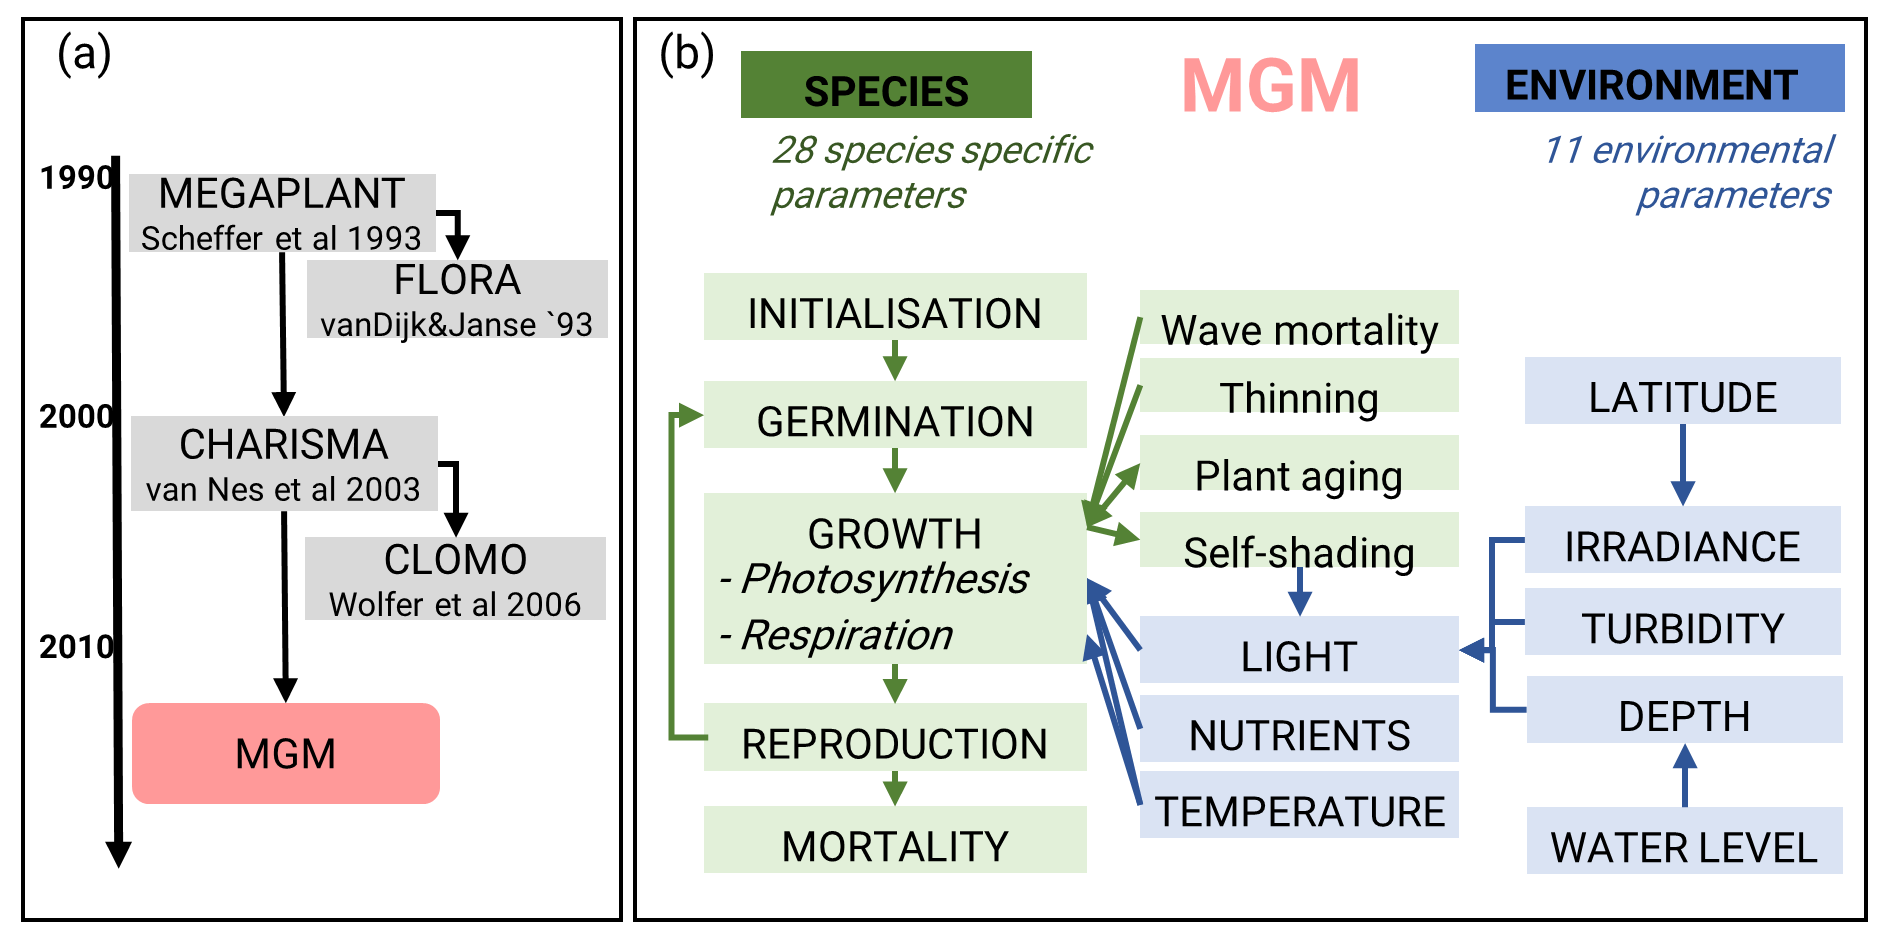
\includegraphics[keepaspectratio,alt={\label{fig:MGM}Model phylogeny of MGM (a) and simplified model scheme (b).}]{_main_files/booklet_pictures/MGM.png}}
\caption{\label{fig:MGM}Model phylogeny of MGM (a) and simplified model scheme (b).}
\end{figure}

Documentation and code is open access on
\href{https://github.com/AnneLew/MGM}{GitHub}.

Further questions: ask Anne

\subsection{metaRange}\label{metarange}

general info - TODO JANA \& STEFAN

\subsubsection{R version}\label{r-version}

TODO Stefan

\subsubsection{Julia Version}\label{julia-version}

TODO Jana

\chapter{Computational methods}\label{computational-methods}

Now, let's come to the more practical part of our Beginner's Guide.
Here, you will get an overview on the methods that we use in our working
group.

\section{Sensitivity Analyses}\label{sensitivity-analyses}

Methods that determine how target variables are affected based on
changes in other variables known as input variables.

\subsection{Overview}\label{overview}

General broad overview in \textbf{Sensitivity Analysis in Practice : A Guide
to Assessing Scientific Models} \citep{saltelli2002}

Comparison of different sensitivity analysis methods: A performance
comparison of sensitivity analysis methods for building energy models
Idea: Run the sensitivity analysis not on the data itself but on a
comparison between data and model (as you would use in the validation)
-\textgreater{} This is the measure to which you want to know the sensitivity

\subsection{Local}\label{local}

= One-factor-at-a-time (OAT)

TODO Anne

\subsection{Global}\label{global}

Morris screening and enhancement as used in the R package sensitivity
(Campolongo 2007).

TODO Anne

\section{Virtual ecologist}\label{virtual-ecologist}

TODO

\section{Parameter optimization}\label{parameter-optimization}

\subsection{Direct methods}\label{direct-methods}

Differential evolution optimization Differential Evolution with DEoptim
(R package) How does differential evolution work?

TODO Anne

\subsection{Bayesian Calibration}\label{bayesian-calibration}

florianhartig/LearningBayes: An introduction to Bayesian statistics
Bayesian Tools - General-Purpose MCMC and SMC Samplers and Tools for
Bayesian Statistics Inverse modeling
\url{https://arxiv.org/ftp/arxiv/papers/2007/2007.15580.pdf}

\subsection{Emulatoren}\label{emulatoren}

Approximieren das Modell selbst ``modelling a model'' / ``meta-model''

TODO

\subsection{Neural networks}\label{neural-networks}

\url{https://arxiv.org/ftp/arxiv/papers/2007/2007.15580.pdf}
\url{https://link.springer.com/chapter/10.1007\%2F978-3-030-44584-3_43}
\url{https://royalsocietypublishing.org/doi/10.1098/rsbl.2017.0660}

Bayesian \url{https://bg.copernicus.org/articles/15/5801/2018/}

TODO

\subsection{Tips and Tricks}\label{tips-and-tricks}

For all methods, first, run an optimization on a dataset that you
produced with the model. That way, you can find out whether the
optimization algorithm can find the parameters with which you modelled
the dataset. This can help to verify that your optimization method
works.

\section{Machine Learning}\label{machine-learning}

If you are interested in machine learning,
\href{https://theoreticalecology.github.io/machinelearning/index.html}{here}
is a course by our colleague Florian Hartig from the University of
Regensburg. This course is held in R.

\section{Phylogenetic Analyses}\label{phylogenetic-analyses}

TODO

\section{Functional Analyses}\label{functional-analyses}

Wright et al (2005) provides a good basis for `trusting' trait-trait
associations above 5-fold variation and/or n=20 spp, within a study
\citep{wright2005}. Although Wright et al.~show trait correlations with as
few as 4 species.

For multivariate analyses:

\begin{itemize}
\item
  MANOVA (because traits are not independent from one another) and
  canonical discriminant analyses (CDA) =Y check R package candisc
\item
  trait network analyses (R package igraph - Csardi and Nepusz, 2006)

  \begin{itemize}
  \tightlist
  \item
    Mantel test for comparing trait correlations across groups (e.g.
    taxonomic, trophic or guild groups)
  \end{itemize}
\item
  PCA (useful for visualization as well)
\end{itemize}

\section{SDMs}\label{sdms}

ToDo: WHAT IS A SDM?

TODO: organize better and make references readable

Tutorials:

\begin{itemize}
\item
  Damaris Zurell: \url{https://damariszurell.github.io/SDM-Intro/}
\item
  Babak Naimi: \url{https://www.youtube.com/watch?v=83dMS3bcjJM}
\item
  \url{https://www.biogeoinformatics.org/}
\item
  Daniel Griffith:
  \url{https://griffithdan.github.io/pages/outreach/SDM-Workshop-OSU-FALL2017.pdf}
\end{itemize}

Further:

\begin{itemize}
\item
  ModestR Software: \url{http://www.ipez.es/ModestR/}
\item
  ModestR Tutorial:
  \url{https://www.slideshare.net/modestrsoftware/21-creating-virtual-species-and-calculating-simple-ensemble-models-with-r-that-can-be-later-used-with-version-modestr-56-or-higher}
\end{itemize}

Earlier models:

\begin{itemize}
\tightlist
\item
  BIOCLIM: \url{https://doi.org/10.1111/ddi.12144}
\end{itemize}

Packages:

\begin{itemize}
\item
  sdm: \url{https://cran.r-project.org/web/packages/sdm/sdm.pdf}
\item
  kuenm: \url{https://peerj.com/articles/6281/}
\item
  virtualspecies \citep{leroy2015}
\item
  \url{https://cran.r-project.org/web/packages/virtualspecies/virtualspecies.pdf}
\end{itemize}

For Maxent type of models:

\begin{itemize}
\tightlist
\item
  Evaluating Maxent niche models with ENMeval:
  \url{https://doi.org/10.1111/2041-210X.12261}
\end{itemize}

For ensemble models:

\begin{itemize}
\item
  Biomod Paper: \url{https://doi.org/10.1111/j.1600-0587.2008.05742.x}
\item
  Biomod2 package:
\item
  \url{https://cran.r-project.org/web/packages/biomod2/biomod2.pdf}
\item
  \url{https://github.com/biomodhub/biomod2}
\item
  ESDM: \url{https://doi.org/10.1111/2041-210X.13283}
\item
  Stacked SDMs (for species richness/diversity):
\item
  SSDM:
  \url{https://cran.r-project.org/web/packages/SSDM/vignettes/SSDM.html}
\item
  Joint-SDMs for co-occurrence data:
\item
  with HMSC: \url{https://doi.org/10.1111/2041-210X.13345}
\item
  sjSDM: \url{https://doi.org/10.1111/2041-210X.13687}
\item
  \url{https://github.com/TheoreticalEcology/s-jSDM}
\end{itemize}

Useful literature:

\begin{itemize}
\item
  Review about SDMs \citep{hao2019}
\item
  ODMAP: A standard protocol for reporting SDMs \citep{zurell2020}
\item
  Correcting sampling bias in MAxent \citep{kramer-schadt2013}
\end{itemize}

\chapter{Project management}\label{project-management}

Apart from all the programming you are going to learn, it might also
make sense for you to learn how to structure your work day/week and your
whole project so that you never lose track of what you need to do, and
what you already have done, and how to do it all efficiently.

\section{Computational Notebooks}\label{computational-notebooks}

These are files that allow you to write descriptive text, code, and the
output of that code. They are particularly useful for:

\begin{itemize}
\tightlist
\item
  learning and teaching coding, because the code and its output are
  shown together, so you always know what does what
\item
  documenting analysis/model development, because, besides the outputs
  of the code you are trying out, descriptive text can help elaborate
  your ideas better, and even include figures or links in the same
  file as the code you are working on.
\item
  sharing computational work: Your collaborator/supervisor will be
  able to follow your reasoning with the descriptive text and check
  your work in the code blocks and its outputs.
\end{itemize}

See the complete tutorial
\href{https://github.com/FellowsFreiesWissen/computational_notebooks}{here}.

\section{Excel-based orga}\label{excel-based-orga}

\href{https://www.biozentrum.uni-wuerzburg.de/cctb/research/ecosystem-modeling/people/anne-lewerentz/}{Anne}
has a very nice Excel sheet that she uses as a calendar. It has an
annual sheet, a weekly schedule, and more. What is nice about this is
that it is not restricted to Outlook has multiple options for sorting,
filtering, coloring, and is completely customizable. Her template is
available upon request :)

\section{Pomodoro timer}\label{pomodoro-timer}

``The Pomodoro Technique is a time management method developed by
Francesco Cirillo in the late 1980s. It uses a timer to break work into
intervals, traditionally 25 minutes in length, separated by short
breaks. Each interval is known as a pomodoro, from the Italian word for
`tomato', after the tomato-shaped kitchen timer Cirillo used as a
university student.'' (From wikipedia)

Using the Pomodoro technique can be helpful if you struggle with feeling
overwhelmed by your workload. Just start with any task and work on it
for the set time (usually 25 minutes), then take a (5 minute) break. You
will be surprised by how much you can get done in just one Pomodoro
session!

You can either set your phone alarm at your chosen intervals, or you can
look up one of the many Youtube channels that provide you with some
background white noise during work periods, and music during the breaks.
\href{https://www.biozentrum.uni-wuerzburg.de/cctb/research/ecosystem-modeling/people/jana-blechschmidt/}{Jana}
likes to listen to this \href{https://www.youtube.com/c/PeacefulAmbience}{ambience
channel}, for example.

\section{Asana}\label{asana}

Basically just on online kanban board. + Its has unlimited projects and
a nice look - proprietary and web based.

\section{Finishing a PhD}\label{finishing-a-phd}

Anne collected (with Selina, FU Berlin) all there strategies that helped
them to finish their thesis:
\href{https://docs.google.com/spreadsheets/d/1A_tDiVdG4E-zXpFXDHKXBJr95RCt3S41GH64gicyOXM/edit?usp=sharing}{Tips\&Strategies}

\chapter{Writing \& Publishing}\label{writing-publishing}

\section{Tools}\label{tools}

\subsection{latex}\label{latex}

Latex is a software to write text. You can find thousands of tutorials
online. If you want to work with latex on shared documents, consider
\href{https://de.overleaf.com/}{overleaf}.

\subsection{Others}\label{others}

Other tools can be:

\begin{itemize}
\tightlist
\item
  Markdown
\item
  Word
\item
  Google drive (for collaboration) \ldots{}
\end{itemize}

\section{Writing Papers}\label{writing-papers}

Here some general tips for structuring and writing a manuscript.

\subsection{Structuring the manuscript}\label{structuring-the-manuscript}

\begin{itemize}
\item
  Find a journal of interest, check the author guidelines and follow
  the instructions. A list of journals of interest can be found in the
  internal folder of the github.
\item
  The manuscript needs to have page and line numbers, double spaced
  lines
\item
  \textbf{Abstract:}

  \begin{itemize}
  \item
    Normally abstracts are around 300 words. For a better abstract,
    structure it in small sections, much like manuscript itself:
    Introduction, Methods, Results, Discussion and conclusions.
  \item
    No references in the abstract
  \end{itemize}
\item
  \textbf{Introduction:}

  \begin{itemize}
  \item
    A ideal introduction has a simple structure without subheaders,
    but with generally 4-5 paragraphs:

    \begin{itemize}
    \item
      First paragraph: Present the key challenge of the
      manuscript, general importance of this challenge for science
      and open questions
    \item
      Second paragraph: Details on what people has already found
      out about the main challenge.
    \item
      Third paragraph: what is the best study system, why and open
      questions
    \item
      Fourth paragraph: what is the best tool or method strategy
      and why. This paragraph may be merged with the third one if
      study system and tool are too intertwined
    \item
      Fifth paragraph: Aims, specific study questions and
      hypotheses, experimental design, expectations. It will help
      the paper structure if you explicitly list with numbers very
      specific questions or hypotheses to be addressed by the
      experiment and analyses.
    \end{itemize}
  \item
    General suggestion: every paragraph must have the first sentence
    presenting the topic of the paragraph and everything related to
    it must be in the same paragraph. If the paragraph is in the
    introduction, the last sentence may be related to an open
    question that will be targeted in your study. If the paragraph
    is in the discussion, the last sentence must be a strong
    concluding sentence with a take-home message based in your
    findings.
  \end{itemize}
\item
  \textbf{Methods}

  \begin{itemize}
  \item
    must have one general, but small paragraph telling what was the
    main methodological approach.
  \item
    Then the methods must be structured in subsections. Typically,
    these are:

    \begin{itemize}
    \item
      ‚Study system' or ‚empirical data' if empirical or ‚Model
      description' is modelling manuscript (with many
      sub-subsections):

      \begin{itemize}
      \item
        For modeling papers, follow the ODD protocol
        \citep{grimm2010}
      \item
        It is also useful to document model development, mostly
        as Appendix, with a TRACE document \citep{grimm2014}
      \end{itemize}
    \item
      ‚Experimental design': this must explain what experiments
      were carrying out to answer i) all the questions; ii)
      particular questions. Normally you have one figure
      illustrating the scenarios.
    \item
      ‚Analyses': Start with a general paragraph explaining what
      model output you used for analyses, whether you did further
      calculations and manipulations for analyses that are
      relevant for all study questions. Thereafter, then follow
      the structure of the hypotheses and create one paragraph for
      study question and explain what analyses were carried out to
      answer explicitly each specific study question.
    \end{itemize}
  \end{itemize}
\item
  \textbf{Results:}

  \begin{itemize}
  \tightlist
  \item
    Start explaining general overall findings, then structure
    according to the study questions/hypotheses. Normally you have
    one Figure for each question.
  \end{itemize}
\item
  \textbf{Discussion:}

  \begin{itemize}
  \tightlist
  \item
    This is where you discuss the findings in relation to one
    another and tot he literature. It is useful to start discussing
    the results in a section per study question. Then add a section
    on implications to theory and conservation. Another section to
    limitations and perspectives. Finally a conclusion.
  \end{itemize}
\end{itemize}

\subsection{Language Tips}\label{language-tips}

\begin{itemize}
\item
  ‚in order' can be always excluded to save words
\item
  Avoid synonyms, define terms at first mention, preferentially in the
  introduction and stick to that term throughout the text! You can add
  a couple of synonyms early in the introduction to increase
  findability of the manuscript in search engines when it gets
  publish. However, for most part of the paper use only one term for a
  given concept.
\item
  You need to edit each sentence. This make sentences simple and
  direct. Prefer only one verb per sentence.
\item
  You cannot use the conjunction ‚On the other hand,'' without having
  used ‚On the one hand,' right before
\item
  In written English, the sentences should always have a noun!!!

  \begin{itemize}
  \tightlist
  \item
    Example: Wrong: „For plants, some traits do this, others do
    that.'' Correct: „For plants, some traits do this, other traits
    do that.''
  \end{itemize}
\item
  In this regard, in any given sentence, there should be only one
  subject to avoid confusion with the verbs.

  \begin{itemize}
  \tightlist
  \item
    Example: Wrong: „Plants have traits and some do this.'' (some
    plants or some traits?) Correct: „Plants have traits. Some
    traits do this.''
  \end{itemize}
\end{itemize}

\section{Rebuttal Letters}\label{rebuttal-letters}

\section{Reviewing Papers}\label{reviewing-papers}

A template of a review feedback letter:

Comments to MS-ID

For editor {[}This section should be cut and pasted onto the part of the
review form online that is confidential to the editor, i.e.~not visible
to the authors, and should NOT be retained in this file if you decide to
upload the comments as a file.{]}:

{[}here you talk in brief your general opinion on the paper and justify
your recommendation, while mentioning in the aspects, like statistics,
that you cannot comment with much confidence. Stress what you think from
all your concerns listed below, which are the most critical, those that
the authors MUST clarify{]}

For authors {[}From this section to the end of the file you can upload to
the online review form, normally only necessary when the comments are
too extensive.{]}:

{[}Here you explain in 1-3 sentences what the paper does and finds
(important for the editor). Explain your general assessment on the
language and style. Whether the authors can substantiate their claims,
whether you see potential in the manuscript, that you may have concerns
and what is your general recommendation. Key recommendations are: reject
(even if the authors tackle the issues, the manuscript might not fit the
scope of the journal, or would remain too trivial and non-original);
reject and invite for resubmission (the manuscript has a potential for a
good contribution to the field if the major points are correctly
addressed, particularly if major points involve re-doing analyses, which
mean potentially changed content after revision); major revision (when
there are major points, but the authors just need to do some re-writing
and/or re-analysing); minor revision (when there is no major point, just
minor corrections); accept (everything is at contempt). Be always polite
and encouraging.{]}

Major points:

{[}Here you list the points that you find critical, which may implicit
mean the authors will need to 1) rewrite; 2) re-analyse; 3) re-do
experiments. Critical points: big flaws in the rationale; non-adequate
experiment or analyses; wrong conclusions; missing analyses; missing key
literature; poor structure. These points can be general and not
necessarily addressed to a particular line or sentence. Be always polite
and encouraging; if you have any critic, you must provide a solution or
a suggestion. Do not criticize just for the sake of it.{]}

Minor points:

{[}These are points that you can locate specifically to a line, sentence,
paragraph, table or figure. Normally these are unclear statements,
typos, errors, missing information, poor design, formatting issues.
These can be normally quickly solved.{]}

\bibliography{book.bib,packages.bib}

\end{document}
